% Activate the appendix in the doc
% from here on sections are numerated with capital letters 
%\appendix

% Change equation numbering format to be sequential within sections in the appendix
\renewcommand\theequation{\Alph{section}\arabic{equation}} % Redefine equation numbering format
\counterwithin*{equation}{section} % Number equations within sections
\renewcommand\thefigure{\Alph{section}\arabic{figure}} % Redefine equation numbering format
\counterwithin*{figure}{section} % Number equations within sections
\renewcommand\thetable{\Alph{section}\arabic{table}} % Redefine equation numbering format
\counterwithin*{table}{section} % Number equations within sections



\begin{appendices}


%--- For single section ---%
%\section*{Appendix}

%--- For multiple sections ---%
% Appendix formatting
\renewcommand{\thesection}{Appendix \Alph{section}}
\renewcommand{\thesubsection}{\Alph{section}.\arabic{subsection}}

%--- Section ---%
\section{Section title of first appendix}
Appendices are used for supplementary material that is relevant to the main text but not essential for inclusion in the text itself—for example, questionnaires, interview transcripts, extended data tables, or equipment descriptions.
\begin{itemize}
\item If there is only one appendix, label it as “Appendix”; if there are multiple appendices, label them as “Appendix A,” “Appendix B,” and so on, arranging them in the order they appear in the paper. 
\item All appendices must be referenced in the main text, and only items that enhance the reader’s understanding or support your argument should be included.
\item Tables and figures in an appendix should be labeled separately (e.g., Table \ref{tab_a1}, Figure \ref{fig:cat2}).
\end{itemize}

%--- Subsection ---%
\subsection{Fist subsection title of first appendix}
As shown in Equation \ref{eq_a1}, the section number is inserted in the equation number.
\lipsum[11]

\begin{equation}
Y_\infty = \left( \frac{m}{\textrm{GeV}} \right)^{-3}
    \left[ 1 + \frac{3 \ln(m/\textrm{GeV})}{15}
    + \frac{\ln(c_2/5)}{15} \right]
\label{eq_a1}
\end{equation}

%--- Subsection ---%
\subsection{Second subsection title of first appendix}
As shown in Table \ref{tab_a1}, the section number is inserted in the table number.

\begin{table}[!ht]
\caption{Sample table with three parts and five columns\label{tab_a1}}
\begin{threeparttable}
\begin{tabular*}{\columnwidth}{@{\extracolsep\fill}lllll@{\extracolsep\fill}}
\toprule
column 1 & column 2 & column 3 & column 4 & column 5\\
\midrule
row 1 & data 0 & data 1 & data 2 & data 3 \\
row 2 & data 4 & data 5 & data 6 & data 7 \\
row 3 & data 8 & data 9 & data 10 & data 11\\
\bottomrule
\end{tabular*}
\end{threeparttable}
\end{table}

%--- Subsubsection ---%
\subsubsection {Subsubsection title of first appendix}
\lipsum[12]


%--- Section ---%
\section{Section title of second appendix}

As shown in Figure \ref{fig:cat2}, the section number is inserted in the figure number.
\lipsum[13]

% figure b1
\begin{figure}[!htbp]
\centering
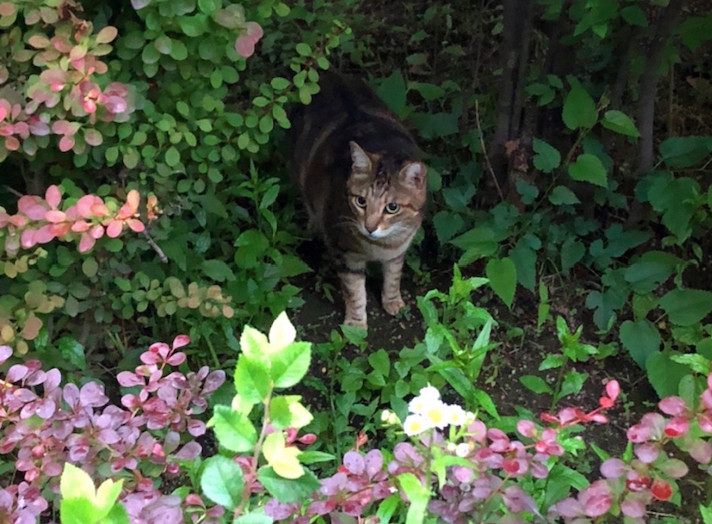
\includegraphics[width=0.8\linewidth]{z_cat_momo_2.jpg}
\caption{\label{fig:cat2}This cat picture is located at the 'figures' folder.}
\end{figure}

\lipsum[14]

\subsection{Appendix subsection title here}
\lipsum[15]

\end{appendices}
